% !TEX TS-program = pdflatex
% !TeX spellcheck = cp1251
% !TEX root = main.tex

\documentclass[a4paper,twoside,11pt]{article}

\usepackage[cp1251]{inputenc}
\usepackage[main=english,russian]{babel}
% !TEX TS-program = pdflatex
% !TeX spellcheck = en_US
% !TEX root = main.tex
\newcommand{\OCanren}{\textsc{OCanren}}
\newcommand{\OCaml}{\textsc{OCaml}}
\newcommand{\Scheme}{\textsc{Scheme}}
\newcommand{\Kotlin}{\textsc{Kotlin}}
\newcommand{\Klogic}{\textsc{Klogic}}

\journalnumber{1}
\curyear{2025}
\authorlist{LOZOV AND OTHERS.}

\title{Constraint Programming for Automatic User Interface Construction}
\titlehead{Constraint Programming for Automatic User Interface Construction}
\headerdef

\udk{004.51}
\rubrika{Software Engineering, Testing and Verification}
\dateinput{\DTMDate{2024-11-0}}

\rusabstr{
% !TEX TS-program = pdflatex
% !TeX spellcheck = cp1251
% !TEX root = main.tex

We approach a task of automatized design of  graphic user interface (GUI) by construction a system based and constraint programming.
It takes designer-specified layout constraints (\emph{guidelines}) and  logical structure of desired interface, and generate layouts,
each of which complies with these guidelines by construction.
The system is implemented as WEB application, and generates results in a real time.
%To
%We describe a system which, given a set of designer-specified layout constraints (\emph{guidelines})
%and a description of graphic user interface (GUI) logical structure generates a set of concrete layouts,
%each of which complies with these guidelines by construction. We give a formal treatment of the task as a
%constraint satisfiability problem and describe the construction of a sound and complete solver
%based on the utilization of \emph{relational verifier-to-solver} approach. We also describe a number
%of refinements which make the solver more efficient and applicable.
%\textcolor{red}{RECHECK}
}

\author{
{\bfseries Lozov~P.~A.$^{a1}$, Kosarev~D.~S.$^{a2}$, Boulytchev~D.~Yu.$^{a3}$, Fokin~D.~S.$^{4}$}
\\ {\itshape $^a$St.~Petersburg State University,}
\\ {\itshape }  {\slshape 7-9} {\itshape  Universitetskaya Embankment,} {\slshape St Petersburg, 199034,   Russia}
\\ {\itshape $^1$e-mail: lozov.peter@gmail.com,} { ORCID: \ORCIDLozov{} }
\\ {\itshape $^2$e-mail: d.kosarev@spbu.ru,} { ORCID: \ORCIDKosarev{} }
\\ {\itshape $^3$e-mail: dboulytchev@math.spbu.ru,} {ORCID: \ORCIDBoulytchev{} }
\\ {\itshape $^4$e-mail:  denis.fokin@gmail.com, no affiliation}
}
%\thanks{~}

\date{\DTMDate{2024-11-0}}

\begin{document}

\maketitle
\setcounter{page}{3}
%%%%%%%%%%%%%%%%%%%%%%%%%%%%%%%%%%%%%%%%%%%%%%%%%%%%%%%
\He{Introduction}
\label{sec:intro}
% !TeX encoding = windows-1251
% !TeX spellcheck = ru_RU
% !TEX root = mainrus.tex

����������� ���������� ������������ (GUI) �������� ����� �� �������� ���������������� �������� �������������� � �����������. ������������ ��������� ����� ����������� ��������� ���������� � ���������� �������� ������� �� ������������ �����������, ���������, ��������� ���������, ����������, ������� �������� � �.�. ������ ������ ����� ��������� ������� ����������� ������: ���������� ����������� ����������� ����������� ������� �������~\cite{UI1}.

������� ������������ �������� �� ��������, ��� ������ ��������� ��������������� � �������. ��� �������� ������������� ���������� ���������� ��������� ��������� ������������, �������������� � ��������������� ��������, ��� ������� ����������� ������, �������� ������������ �������� �� ������. � ���������� ��������� �� ������ ��������� ��� ������������� ����������� (UI), �� � ��� ������������ �� ����������������� �������������� (UX)~\cite{UI5}, ������� ������������� ������� (����. guidelines) ��� �������� ����������� �����������. ��� ������� ����� ����������� ���������, �������������� � �������������, � �� ���������� ������� ����� � ��������, ������� ����� �� ���� � �������������. �������������� ����� �������������� � ����������� ����� ������������ ���������� � ����������, �������� � ��������~\cite{UI6}. ����� ����, ���������� ������� �� ������ ����� ��������� � ��������� ����������� � ����������� �������. ������� ������������� �������� ���������� ��������� ���������� ������� ������ �������������� ����������� ������������.

� ������ ������ ����������� ������ � ������� ������������ (����. layout) ��������� ���������� GUI � ������ ������ ������ �������������� �����������. ���� ������ GUI ��������� ���������� ��������� ��������� ���������� (��� ����� ��� �������������) � ���������� ������������ ���������, �������� � ������������ (����� �������� ����������). �� ����������� ������������������ ������, �������, ����������� �� ���������� ��������� (��������������� �������������) � ������ ������ (��������������� ����������), ����������� ������������ ��������� ���������� � ������������ � ����� ���������. ��������� ������� ����� ���� ��������������, ����� ������������ ��������� ��������� ������������, ��������������� ��. �� ������������� ������ ����������� ��� ������ �������������� ����������� (����. constraint satisfaction) � ���������� ����������� ����������������~\cite{TRS} � ����� \enquote{�����������-��-��������}~\cite{searchproblems} (����. verifier-to-solver) ��� �������� ��������, ������� ����������� �������� ���������� � ������� ����������. � ����� ����������� ����� ���� �������� ����������� �������������, ������� �� ��������� ��� ����������� (������� �������������), ����� �������� ��� ������������������. � ���������� ��������� ��������, ������� ������� �� ����� ������������ � ��������������� ����. ����� ����� ���������� ������������ ������������� � �������� ����������� �� ���������� � �������� � �������������� SMT �������� Z3~\cite{Zthree}, ��� ��������� �������� ���������� ���������� ���� ��������� ����������. ���� ������ ��� ����������� ������� ���������� � ������ ��������: �� ������ ��������� ���������� ��������� �� ����������� ��� ������������ ���������, ��������������� ������������ ��������.

��� ���� �������� ���������� ����������, ����� �������� �� ������� ��������.

\He{GUI Model}
\label{sec:scene}
% !TEX TS-program = pdflatex
% !TeX spellcheck = en_US
% !TEX root = main.tex

In this section we present a simplified GUI model which incorporates all important features of the
domain. In the real implementation this simplified model is extended a little bit, but this extension
does not introduce any essential changes into the synthesis algorithm.

We can identify three important aspects of GUI: a \emph{structure}, a \emph{layout}, and a \emph{guideline}.
\emph{Structure} describes the set of GUI controls and their relations; \emph{layout}, on the other hand, determines
their relative placement. This approach aligns well with a common tendency to introduce a separation between business
logic and its visual representation~\cite{UI3}. A \emph{guideline} maps certain controls of a structure into some concrete
layout primitives.

We demonstrate these notions with the following example. Let us have a GUI form shown in Fig.~\ref{form1}. We can describe its structure as follows:

\begin{itemize}
\item there are three GUI controls: a check box, a text label, a drop-down list (combo box);
\item there is a dependency relation between the text label and the combo box since the former \emph{describes} the
  latter; thus, the text label and the combo box constitute a compositional entity;
\item there is an order relation between the checkbox and this compositional entity
  since (as we speculate) there is an implied dependency caused by the importance of the components
  from the perspective of the GUI author.
\end{itemize}

We can depicture this structure as shown in Fig.~\ref{form1-structure-layout}\subref{form1-structure}.
Thus, we can treat a structure as a set of named \emph{relations} between controls (and, possibly, other
data domains such as strings, numbers, etc.). In our approach we divide all such relations into two categories~---
\emph{abstract} and \emph{concrete}. The semantics of \emph{abstract} ones is assigned by a guideline, \emph{concrete}~---
by the system. Concrete relations describe the types of the controls, their various properties (the contents of
text fields, sizes, etc.); they also can be used to combine other controls into ordered or unordered groups or
\emph{virtual controls}~--- containers which incorporate other controls and behave as a whole.

The set of \emph{abstract} relations contains such relations as binary ordering (one control after another), description (one
control contains a description of another, like a label of a check box or text field, etc.), subordination (one control can
be considered as a ``subordinate'' of another, for example, a text field, enabled by a checkbox). But actually these
relations are just conventional abstract names which can be used both in structure descriptions and guidelines. Their
semantics is completely determined by a guideline, and the system does not contain any specific treatment of
these relations. End-users can freely add custom abstract relations and define their semantics in the guidelines.

For a given structure its \emph{layout} can be specified using a set of primitives describing the placement
of controls, their alignment and other similar properties. In the given example the label and combo box are
laid out horizontally next to each other with a certain horizontal inset, the checkbox is stacked over the compositional
label and combo box pair with a certain vertical inset, and the whole layout is left-justified. We can depicture the
layout in question as shown in Fig.~\ref{form1-structure-layout}\subref{form1-layout}. Unlike relations used for
describing structures, all primitives of layout description have a hardcoded semantics which the
synthesis algorithm relies upon.

Finally, a guideline contains a set of rules prescribing what layout primitives should be used for
certain (sub)structures of GUI under certain conditions. In Fig.~\ref{form1-structure-layout}\subref{gdrule}
we show an example of such a rule, taken from \textsc{JetBrains} set of conventional GUI guidelines~\cite{JBG}.
As a rule, GUI guidelines are described in informal terms using a number of examples; in the next section
we present their formal treatment.



\begin{comment}
In our simplified model a structure is completely invariant w.r.t. layout: regardless what a layout could
be the assortment of controls and their logical/functional dependencies remains the same.


We consider connected structures only where each control is related to some other. If the structure can be divided into several
unrelated parts, each of them is laid out independently with possible overlapping.

%Reiterating the example in the Fig.~\ref{form1}, we can now provide a more concrete description of
%its GUI structure (see Fig.~\ref{form1-concrete-structure}).

%From the GUI structure point of view these relations are considered as fully abstract entities. Their semantics
%and impact on the layout is determined by the layout guidelines only.

\subsection{GUI Layout}
\label{constraints}

We have identified the following set of layout primitives:

\begin{itemize}
\item vertical composition of controls (control $C_1$ is laid out directly on the top of the control $C_2$):
  \[
     \term{vert}\,(C_1,\,C_2)
  \]
\item horizontal composition of controls (control $C_1$ is laid out directly to the left of the control $C_2$):
  \[
     \term{hor}\,(C_1,\,C_2)
  \]
\item vertical alignment of controls (does not affect the horizontal position of controls):
  \[
     \term{valign}\,(C_1,\,C_2)
  \]
\item horizontal alignment of controls (does not affect the vertical position of controls):
  \[
     \term{halign}\,(C_1,\,C_2)
  \]
\item horizontal indentation of one control to another:
  \[
  \term{indent}\,(C_1,\,C_2)
  \]
\end{itemize}

%This is a somewhat simplified model; in reality the additional arguments should be specified for these primitives which
%describe the \emph{insets} and \emph{alignments} of the controls being laid out. An inset specifies a desirable vertical
%or horizontal space between controls; as for alignments, different kinds of those are distinguished: top, center, bottom,
%and baseline vertical alignments, and left, right, and center horizontal alignments. As for now we consider the insets
%being a predefined constants and limit the alignments to some default ones; we argue that this choice does not
%undermine the approach we describe.

\begin{figure}[h]
  \centering
  \scalebox{0.8}{
  \begin{tikzpicture}
    \node[rectangle,draw,minimum width=3.1cm,minimum height=1cm] (A) at (1.6, 1.4) {A};
    \node[rectangle,draw,minimum width=1cm,minimum height=1cm] (B) at (0,0)        {B};
    \node[rectangle,draw,minimum width=2cm,minimum height=1cm] (C) at (1.6,0.2)    {C};
%    \path[draw,dashed] (1.6, 0.7) -- (4, 0.7);
%    \path[draw,dashed] (1.6, 0.9) -- (4, 0.9);
%    \path[draw] (3.8, 1.3) -- node[above] {\emph{pad}} (3.8, 0.3);
  \end{tikzpicture}}
  \caption{Layout example}
  \label{layout-example}
\end{figure}

This primitives can be independently used for different controls: for example, controls $A$ and $B$ can be composed
vertically, $B$ and $C$~--- horizontally, and $A$ and $C$ can be horizontally aligned by center, which would
provide the following layout (see Fig.~\ref{layout-example}). Note, the constraints in this example do not require
$B$ and $C$ to be aligned \emph{vertically}.
\end{comment}

\FloatBarrier

\clearpage
\He{Layout Synthesis as a Constraint Satisfaction Problem}
\label{sec:guidelines}
% !TeX encoding = windows-1251
% !TeX spellcheck = ru_RU
% !TEX root = mainrus.tex

� ����� ������ ���������� ���������, ���������� � ���������� �������, ����������� ��� ����� ��������� �� ��������� ��������� ��������� ���������� $\mathcal{C}$.
���������� ���� ��������� $\Sigma=\{r^{n_i}_i\, |\, r^{n_i}_i\subseteq\mathcal{C}^{n_i}\}$ ��� ��������� ���������, ���    $r^{n_i}_i$ �������� \mbox{$n_i$-�����} ���������� ��� $\mathcal{C}$;
��� ������ �������� �� ����� ������������� ����� ���������, ��� ������, ��������� ���������� ��������� ���������� � �.�.

%In our model given in the previous section the logical structure of GUI is described by
%a number of relations between a certain set of controls. Let $\mathcal{C}$ be a set of
%controls and let a structure $\Sigma=\{r^{n_i}_i\, |\, r^{n_i}_i\subseteq\mathcal{C}^{n_i}\}$ be a set of
%relations, where $r^{n_i}_i$ is an \mbox{$n_i$-ary} relation on $\mathcal{C}$; without loss
%of generality we do not consider property-like relations like size, text contents, etc.

\emph{����������� ��������} ����� �������� �������������� ����� $r^n\,(X_1,\dots,X_n)$, ��� $r^n$ --- ��� $n$-����� ��������� � $X_j$ --- ��� ������������� ��������� ����������.

%A \emph{relational pattern} is a syntactic form $r^n\,(X_1,\dots,X_n)$, where $r^n$ is $n$-ary
%relation and $X_j$ are variables (not necessarily distinct).

\emph{�������� ������������} ������� �������������� ����� $l\,(X_1,\dots,X_n)$, ��� $l$~--- ��� ��������� ������������, � $X_i$~--- ����������.

%A \emph{layout template} is a syntactic form $l\,(X_1,\dots,X_n)$, where $l$ is a layout primitive and
%$X_i$~--- variables.

��� $s\,[X_i\gets c_i]$ ����� ���������� ��������� ����������� ��������� ����������
$c_i\in\mathcal{C}$
������ ���������� $X_i$ � ����������� ������ ��� � ������ ������������  $s$. ����� $\mathcal{FV}\,(s)$~--- ��� ��������� ���� ���������� � ����������� ������� ��� � ������� ������������ $s$, � ����� �������� \emph{����������� ������������} ������ ��� ����������.

%We denote $s\,[X_i\gets c_i]$ the result of substitution of controls $c_i\in\mathcal{C}$
%for variables $X_i$ in a relational pattern or layout template $s$, $\mathcal{FV}\,(s)$~--- the set of all
%variables in a relational pattern or layout template $s$, and call \emph{layout instance} a layout
%template with no variables.


����� $r^n\,(X_1,\dots,X_n)$~--- ��� ����������� ������. ���� ��� ���������� ������ ��������� ���������� $c_1,\dots,c_n\in\mathcal{C}$ ����� %\footnote{\textcolor{red}{���-�� ����� �.������ �������� ��� ����� � �������.}}
$(c_1,\dots,c_n)\in r^n$, �� ����� ��������, ��� ��������� ����������� $r^n\,(X_1,\dots,X_n)\,[X_i\gets c_i]$
%Let $r^n\,(X_1,\dots,X_n)$ be a relational pattern. If for some controls $c_1,\dots,c_n\in\mathcal{C}$
%\[
%(c_1,\dots,c_n)\in r^n
%\]
%
%\noindent  �� ����� ��������, ��� ��������� �����������
%\[
%r^n\,(X_1,\dots,X_n)\,[X_i\gets c_i]
%\]
%\noindent
\emph{�����������} � ��������� $\Sigma$. %(����������, ��� $r^n$ --- ��� $n$-����� ��������� ��� ���������� ����������).
%\textcolor{red}{����� ����� ���-�� ��� �����������??.}


\emph{�������} (�����������) ����� ���������� ���
\[
p_1,\dots,p_k\mapsto l_1,\dots,l_m,
\]


\noindent ��� $p_i$~--- ����������� �������, $l_j$~--- ������� ������������.
����� ���������, ����� ����� ���������� � ������ ����� ���� �� ��� ����������� � �����. �����������, ������� �������, ��� ���� ��������� �������� ���������� ��������� ������� ����������� � ���������, ��  ��� ��� ������ �������������� ������������ ��������� ������������.

%We stipulate that any variable in the right-hand side of a
%rule has an occurrence in its left-hand side; no other restrictions are assumed. Informally a guideline rule says that if
%some controls are related in a certain manner in the structure then a specific layout primitives for (some of) these
%controls can be used.

�����������, ��� ���� ��������� $\Sigma$ � ��������� ����������� ������������ $S$.
����� ��������, ��� ��� ��������� \emph{��������������} ������� ������
  \emph{R} ����� � ������ �����, ����� ��� ������� �������� ���������� $l^*\in S$


%Let us have a structure $\Sigma$ and a set $S$ of layout instances. We say that this set is \emph{confirmed} by a set of
%guideline rules \emph{R} iff for each control $l^*\in S$

\begin{enumerate}
\item ���������� ������� $p_1,\dots,p_n\mapsto l_1,\dots,l_i,\dots, l_m$ � $R$, ����� ���
  $l^*=l_i\,[X_j\gets c_j]$  ��� ���������
  $\{c_j\}\subseteq\mathcal{C}$, ��� $\mathcal{FV}\,(l_i)=\{X_j\}$;

\item ��� ���� ���������� $\{Y_1,\dots,Y_t\}=\mathcal{FV}\,(p_1,\dots,p_n)\setminus\mathcal{FV}\,(l_i)$ ���������� �������� ����������
$c^\prime_1,\dots,c^\prime_t\in\mathcal{C}$ �����, ��� ��� ���� $j$ ����������� \mbox{$p_j\,[X_r\gets c_r,\dots,Y_s\gets c^\prime_s]$}
   ����������� � ��������� $\Sigma$;

\item \mbox{$l_j\,[X_r\gets c_r,\dots,Y_s\gets c^\prime_s]\in S$} ��� ���� $j$.

\end{enumerate}

����������� ���������, $R$ ������������ ��������� $S$ ����� � ������ �����, �����  ��� �������� ���������� $l^*$
����� ���� ��������� �������� �� ������ $R$. ��� ��������, ��� ������ ���� �����-�� ������� � �������� ������������ $l_i$, ������� ����������� � $l^*$ � ������� ��������� �����������  ���������� $X_i$. �� � ���� ������� ����� $X_i$ ����� ���� ������ ���������� $Y_j$.
���� � ��� ��� ���������� ����� �����������, ������� ��������� � ������������ ���������� $X_i$, �������� ��� ����������� ������� ����� ����������� �  $\Sigma$,
����� ������� ����� ���� ��������� � $l^*$ ��������.
� ���� ��, �  ������ ����� ����� ���� ������ ������� ������������, � ���� � ��� �������� ���� �����������,
�� ���� ��������� ������������ ������ ���� �������� � $S$.


%Informally speaking a set $S$ is confirmed by $R$ iff each its control $l^*$ can be properly
%derived according to $R$. This means that there should be some rule containing
%layout template $l_i$ which is turned into $l^*$ by some substitution of its
%variables $X_i$. However, in this rule there potentially can be other variables $Y_j$ besides $X_i$.
%If there exists a substitution for them which, together with the substitution for $X_i$, makes all
%relational patterns in the left-hand side to occur in $\Sigma$, then the rule can be
%applied and $l^*$ can be derived. Finally, as there can be other layout templates in the
%right-hand side of this rule, they will be derived as well, and thus corresponding
%layout instances have to be included in $S$.

������������� ��������� �������� � ���� \emph{���} ������������, ������� ����� ���� ���������� ���������.
��� ��������� �� �������� ������ ������������. ������ ������������� ������������ ��������� ���������� �� ������ ��� ������������� \enquote{�������} � ����� ������ ���������. ������ ��������� ������ ��������������, �� ���� �� ��� ����� ������� �������� ������������� ���������. ��-�� ����� ��� ���������� ������ ��� ���� �������: \emph{��������}.

%Confirmed sets represent all layouts which can be justified according to the guidelines in the sense that they
%do not contain ``extra'' layout instances appeared out of thin air. However being confirmed does not
%necessarily mean to be a ``good'' layout in the sense a regular designer would imply. Indeed, an
%empty set is always confirmed, but can hardly be considered as a valuable layout. Thus, we define
%another property: \emph{coverage}.

����� ��������, ��� ���������� ������������ $S$ \emph{���������} ��������� $\Sigma$ ����� � ������ �����, ����� ��� ������� �������� ���������� $c\in\mathcal{C}$
���������� ��������� ������������ � $S$, ������� ��������� $c$, �.�. �������� $c$ ��� ��������. �������� ����������� ����������, ���  �� ���� ������� ���������� �� ��������� �� ������� �� ���������� � ������ ������������.

%We say that a set of layout instances $S$ \emph{covers} a structure $\Sigma$ iff for each control $c\in\mathcal{C}$
%there is a layout instance in $S$ which binds $c$ (i.e. contains $c$ as a parameter). Coverage
%informally means that no control of a structure is left ``unaddressed'' by given layout.

��������� ������������� ������������ � ��������� ������ ������������� ���� \emph{����������} ������������� � ������ ������,
� �������� --- �������. ������ �� ����������� �� �������� ���� ������� �����, ����� ����� �� ����������� � ����� ������������ ������.

%Confirmed sets in some sense correspond to \emph{sound} layouts w.r.t. to guidelines while covering~--- to
%\emph{complete}; however we refrain from calling them such since we reserve more conventional meanings of these terms.

��������� ���������� ���������� ���, ��� ������� (�����������) ������ �����������, � �� ��������������.
����� �������� �������������� � �������� ��������� $S$ \emph{������������} ����� � ������ �����, ����� �� ���������� ��������������� � ��������� ���������  $S^\prime$, ��� $S\subset S^\prime$.
%The next requirement comes from an observation that guideline rules are expected to be applied, not ignored. We
%call a confirmed and covering set of layout instances $S$ \emph{maximal} iff there is no
%confirmed and covering set $S^\prime$ such that $S\subset S^\prime$.

�������, ������������ ����� ��������� ���������. ��������, ���� ������� $A$ ������ ���� ���������� ������ $B$ � ��������, ��, ��������, ��� ���� �������� ������������ �����������. ����� ���� ���������� ����� �������� ���������:

%Finally, layouts can contain conflicts. For example, if a layout says that a control $A$ has to be put on
%the top of control $B$ and visa versa then, obviously, it is unusable since these two primitives introduce
%incompatible constraints. Among the conflicts we can identify the following:

\begin{itemize}
\item �� ������ ���� ������, ������������ ������ �� ���������� ������������ ��� ������������ (��������������) ����������.
\item �� ����� ������ �������� ���������� ������ ������������� ������ ������/����� �� ������� �������� ����������.
��� � ���������� ���������� ����������� �� ����, ��� ���������, ������������ �� ���� ����������, ������ ���� ��������� ���������.

\item ���� ��� ����������� ��������  ���������� ����������� �������������,  �� ������� ��� �������� ���������� ������ ������ �  ������� �� ������ ������������� �����������. ���������� ��� ����������� ������������� ����������� ��������� ����������.
\item ������� ��� �������� ���������� �� ����� ���� ����������� ������������ � �����������, � ������������� ������������ ���� �����.
\end{itemize}

%\begin{itemize}
%\item There should be no loops or branching comprised of layout primitives for vertical and horizontal composition. This
%  requirement originates from the observation that the relations introduced by these
%  primitives have to be unions of linear orders.
%\item If two compositional virtual controls are laid out horizontally then there should not be
%  controls within both of them which are laid out vertically; symmetrically for vertically
%  laid out virtual controls.
%\item No two controls can be laid out vertically and horizontally at the same time.
%\end{itemize}

��� ��������� ��������� ��-�� ����, ��� �� ����������� �������� ���������� �� ��������� ���������.
����� ��� ������ � ������ ���������, ������� �� �������� ��� ��������� ���������.
����� �������� ��������� ����������� ��� ���������� \emph{�����������}.

%These conflicts originate from the fact that we actually place the controls on a two-dimensional plane.
%There are actually other cases which we omit here for space considerations. We call a set of
%instances \emph{compatible} iff it does not contain conflicts.

�����, ��� ��������� ��������������, ����������� ��������� � ���������� ������������ � ������ ��������� ������ ������. ����� �������� ����� ������������ \emph{�����������}.

%To summarize, we are interested in confirmed, covering, maximal and compatible layouts w.r.t. a given
%set of guideline rules. We call such layouts \emph{sound}.

����� �������� ������ ������������������ ������� � ������ ������. ����� ��������, ��� ���������� ����������� ������������~--- � ����� ������ NP-������ ������.
��� ������������� �����, ���������� ������� NP-������ ������~\cite{GareyJohnson1979} ������ ������������ ���� � ����� � ������� ������ �������.
��� ������������� ��������������� ����� ����� ��������� ���������, � ������� ���� ������� ���������� ������������� ����� ������� �����,  � ��������� �������� ��������� $E$~--- �����. ����� ���������� ����� ������� ������������:
%It is worth mentioning the worst-case complexity of the problem in question. First, it is rather
%easy to see that finding if there exists a sound layout is $NP$-complete in general case.
%Indeed, given an undirected graph we can construct a structure where controls correspond to its nodes
%and some binary relation (call it ``$E$'') corresponds to edges. Then we take the following guideline:
\[
\begin{array}{rcl}
  E\,(x,\, y) & \mapsto & \mbox{hor}\,(x,\, y)\\
  E\,(x,\, y) & \mapsto & \mbox{hor}\,(y,\, x)
\end{array}
\]

����� ���������� ������������ � ������ ������ �� ����������� �������� ��� �������� ���������� (�.�. ���� �����) � ������ ��������� ������������ ���� ``\texttt{hor}'', ��� ������ ��������� ��������� ������������� ������ ����� � �����. ��� ��� ��������� �� ����� ������������ ����, � ������ ������� ���������� ����� ���� ������ ������ ������ � ����� ������ ���������, �� ����� �������� ����������� ����.
%Any sound layout w.r.t. this guideline by definition contains all controls (i.e. nodes of the graph) and
%only layout primitives ``\texttt{hor}'', each of which corresponds to exactly one edge of the graph. Since
%``\texttt{hor}'' can not branch or loop, these edges form a Hamiltonian path.

� ������ �������, ����� ��������, ��� ���������� ���� ���������� ������������ � ������ ������ ��������������� ������� �� ������� ���������.
� ������ ���� ���������� ������������ � ������� �������� �������� ��� �������� � ������ ������ ���������������.
%On the other hand, it is rather easy to see that the number of all sound layouts can be worst-case
%exponential on the size of a structure. As we are aimed at enumerating them all the solvers for
%the problem would inevitably run in worst-case exponential time.




\He{Relational Programming, Verifiers and Solvers}
\label{sec:rel}
% !TEX TS-program = pdflatex
% !TeX spellcheck = en_US
% !TEX root = main.tex


The implementation of our layout synthesizer employs the techniques of relational programming. Here
we briefly recollect what relational programming is and how the approaches and tools we use work.

Relational programming~\cite{TRS} is an approach based on the idea of describing programs as relations. 
It can be considered as a branch of logic programming in which the use of
all non-relational constructs (side-effects, extra-logic features) is discouraged. 
In a narrow sense relational programming amounts to writing programs in \textsc{miniKanren}~--- a specifically designed for this purpose embedded DSL.
Initially developed for \textsc{Scheme}/\textsc{Racket}
\textsc{miniKanren} later was ported for dozens of host
languages\footnote{\url{http://minikanren.org/\#implementations} (accessed: \DTMDate{2024-11-14})}.
We, specifically, use a strongly typed \textsc{miniKanren} implementation for \textsc{OCaml}~\cite{ocaml}, called \textsc{OCanren}~\cite{OCanren}.
\textsc{miniKanren} uses the same theory of Horn clauses as \textsc{Prolog} but with a different
concrete syntax with explicit unification, conjunction, disjunction and fresh variable introduction, and
employs a different \emph{interleaving} search strategy~\cite{interleaving}, which is known to be complete~\cite{certified}.
Besides unification with occurs-check, enabled by default, \textsc{miniKanren} can be equipped with other
basic constraints like disequality constraint~\cite{disuni}, finite-domain constraints~\cite{cKanren}, or
constructs of nominal logic~\cite{aKanren}.

In the context of our work the most valuable property of \textsc{miniKanren} is its capability of expressing \emph{reverse computations}.
It is well-known~\cite{SemanticsModifiers,SemanticsModifiers1} that some complicated programs can be constructed as
the results of inversion of some other, much simpler, programs. 
In particular, a \emph{solver} for a
certain search problem can be considered as an inversion of its \emph{verifier}; it is rather a matter of common knowledge that verifying a
solution is, as a rule, much easier than finding one. 
The relational nature of \textsc{miniKanren} makes
inverse computations particularly easy~\cite{searchproblems}, which opens a way for program
synthesis~\cite{Untagged,WBirdSeven,PatternMatching}.

%Another component of our approach is \emph{relational conversion}. In many cases (but not always!) it is easier to obtain a relational specification
%from functional program than writing the one by hands. We use a tool, called \textsc{noCanren}, which converts programs written is a reasonable
%subset of \textsc{OCaml} into correct-by-construction\cite{conversion} \textsc{OCanren} specifications.

We demonstrate the roadmap of our approach by the following observable example. Let us have a program
shown in Fig.~\ref{fun_vs_rel}\subref{funadd} which concatenates two lists,
and its relational counterpart (Fig.~\ref{fun_vs_rel}\subref{reladd}).
Comparing both of them we can notice that pattern-matching was replaced by disjunction (\lstinline[language=ocanren,basicstyle=\small]|conde|)
and unification (\lstinline[language=ocanren,basicstyle=\small]|===|), data-flow dependent computations with conjunction (\lstinline[language=ocanren,basicstyle=\small]|&&&|),
and fresh variables can be allocated when needed; the postfix ``o'' is traditionally used to distinguish relational definitions. 
Unlike its functional
counterpart the relational specification has \emph{three} arguments \lstinline[language=ocanren,basicstyle=\small]|xs|, \lstinline[language=ocanren,basicstyle=\small]|ys|,
and \lstinline[language=ocanren,basicstyle=\small]|zs|, each of which can contain fresh (initially undefined) variables.
The evaluation of construction \lstinline[language=ocanren,basicstyle=\small]|run$^*$ {appendo xs ys zs}| returns all substitutions for these
fresh variables which make the relation $\{(\mbox{\texttt x}, \mbox{\texttt y}, \mbox{\texttt z})\in\mathbb{N}^3\, |\, \mbox{\texttt x++y=z}\}$ hold, represented as a \emph{lazy stream of answers}. This stream can
then be inspected in a host functional application to retrieve individual answers. 
Thus the same specification can be equally used for concatenation,
prefix removal or decomposition of a list into two sublists.

\begin{figure}[t]
  \begin{subfigure}[t]{0.5\textwidth}
  \begin{lstlisting}[language=ocanren,basicstyle=\small]
   let rec add x y =
     match x with
     | O    -> y
     | S x' -> S (add x' y)
  \end{lstlisting}
  %\vskip12mm
  \caption{Functional addition}
  \label{funadd}
  \end{subfigure}
  \begin{subfigure}[t]{0.5\textwidth}
    \begin{lstlisting}[language=ocanren,basicstyle=\small]
  let rec add$^o$ x y z = ocanren {
    x === O /\ z === y \/
    fresh x', z' in
      x === S x' /\
      z === S z' /\
      add$^o$ x' y z'
  }
    \end{lstlisting}
    \caption{Relational addition}
    \label{reladd}
  \end{subfigure}
  \caption{Functional vs. relational addition of Peano numbers}
  \label{fun_vs_rel}
\end{figure}


\He{Synthesis of GUI}
\label{sec:synthesizing}
% !TeX encoding = windows-1251
% !TeX spellcheck = ru_RU
% !TEX root = mainrus.tex

� ������ ������� ������ ������ ����������� ������������ �� ������ �����������, ������� ����������
���� ��������� �������� ������������ � ���������� ��������� �����������.

����������� ������� ����������� ����������, ���� ������������� �������� ��������, ������������ � ������������� ������� �� �������~\ref{sec:guidelines}
������������ � ���� ���������, ������� ��������� ��������� � ���������� ������������.
�������� ����� ��������, ������ ��� ��������� ������������, ������� ��� ������������� �������� ���������� � ���������, �
��������, ��� ��� ������������� ��������� ���� ������������� ��������� ���������� � ���������. ������������ ����������� ����������, �� �����������.

��� ������������� ��� ����� ������ ��� ��������� ������������ � ����������� ������ �� ���.
��� ������� ��������� ������� �����������.
��������, ���������� ��������� �������:
\[
\term{describes}\,(X,\,Y)\,\mapsto\,\term{vert}\,(X,\,Y),\,\term{halign}\,(X,\,Y)
\]

\noindent ��� ���������� ��������� ������ ��� ��������� ������������� ��������� $\Sigma$ � ������ ����������� ������������  $S$:
%It determines the following (sub)cases for the confirmation check procedure for a structure $\Sigma$ and a set of layout instances $S$:

\begin{lstlisting}[language=ocanren,basicstyle=\small]
 if $\term{vert}\,(X,\,Y)\in S$
 then $\term{describes}\,(X,\,Y)\in\Sigma$ /\ $\,\term{halign}\,(X,\,Y)\in S$
 else if $\term{halign}\,(X,\,Y)\in S$
 then $\term{describes}\,(X,\,Y)\in\Sigma$ /\ $\,\term{vert}\,(X,\,Y)\in S$
\end{lstlisting}

�� �� ��������� \emph{��������������} � ���������� ������������, ��� ��� ��� ����� ������������ ���������� ������������ ����������������.
�������������� ����������� ������ �������: �������� ������������ �� ���������� ��������� �
�� \emph{��������� ����������} �� ����� ���������� ����������� ������������.
�� ���� ������� ������ \textsc{miniKanren} ������ ��� ��� ���������, ������������  ����������, �������� � �������������.
�����   ����������� �� ������������.

�� ���� ������ ��� ��������, � ������� ������ ������� ����������, � �������� ����� ������� ��� ����������.

��-������, ������������� ����������� ������� �� ��������� ������, ������� ������ ��������� ������������.
������� ���������� � ������� ������� ����� �������� ���������� ����� ������������� �������, ������������� �������� ���������� ������������ � ���������.
��� ������� ���� �������� ��� ���������� ��� ���������� \emph{��������}~--- ��������� ������, ������� ���������� ������� �����, ��� ��� ������ ����������� ����������.
��� ������ ������ ��� ����� ������ ��������� �������, ��� ��� ��� ���� ���������� ������������ � ���������� ��������� � ��������� �������� ������.

��-������, ����������� ���������� ��������� ������������ ���������� ��������� ����������� ������������, ����� ������� \emph{�������}, ���� ���� ������������� ������ ������������� � ��������.
����� ��� ���������, ������������� ������������ ������������ ������������, � �� ���� �������� ��� ���������� ���� ������ ����������
� \emph{�������������������} ������ ������������ ������ ������, ������� �������� ���������.
����� ������ ���� ��� ��������� ���� ������������ ���������� ������������.
��� �������� ����������� �� ���� ����, ��� ������������� ���������� ������������ ������, ��� �� �������������, � ������� ����� �������� � ������������������ �������� ��� �������������, ��� ����������������� ������ ��� �� �������������.

������ �� ��� ����� ��������� ������������ �� �������������   ������������   ���������� ��� ��������� ����������� ����������.
%
%Our initial solution generate all compatible sets of instances. However their number can be huge even if
%only confirmed and covered sets are considered. In order to make our synthesizer applicable we have to eliminate
%this overhead. We do this using greedy approach: instead of enumerating all compatible layouts and
%filtering out non-maximal ones we first build one maximal but not compatible layout, then identify all conflicts and,
%finally, eliminate the conflicts by \emph{nondeterministically} canceling minimal numbers of rules
%which introduce these conflicts. This approach gives us a set of all maximal compatible layouts.
%Each of these steps is implemented as an independent relational component.

�� ������ ����   ����������������� ��������� ��� ������� �����������, ����� �������� ������������ (��������, ������������)  ��������� ����������� ������������, �������������� ����������.

%On the first step we non-deterministically apply all guideline rules and combine them into the maximal
%(but probably non-compatible) set of layout instances represented as a hypercube.

�� ������ ���� ������������� ������ ����������� �������������, ����� ����� ��� ���������. ��� ������� ���� ��������� ��������
����������� �����������, ������� �� ��������� � ������ ����������� ������������ ���������, ��� �������� ������ ���������� � ��������� � ������������� �������� �������� ���������������� ����.
������������ � �������� ����������� �� ���������� ��������� ����������� ������ ����� ����������� ������������, ������� �������� �������� ���������������� ����. ������ � �������� ����������� ���������� ������������� ���� ��� ��� ������������� ������ �����������.

%Being run in the reverse direction for a ground hypercube and free variable this verifier returns all
%sets of layout instances which occur in the hypercube and constitute a conflict of given kind. Running a disjunction
%of all such verifiers in the reverse direction gives us the set of all sets of conflicting layout instances.

�� ������� ����   ��� ������� �������������� ������������ ��������� ���������, ��� ���� ��� (��� ������� ������) ��������� ������������ ���������� ������������.
������� ��� ��������� �������. ��������� ��������� ������������� ����������� ���   $S$.
������ ��������� �������� ����� ���������, ����� ������ ���� �������� ������������.
�������, ����� ��-������ ���������� ���������� �� $S$ � ��������, ����� ��������� �����������.
����������� ������ ��������� ����� ��������� ����� ��������� ����������.
���   ������� ������������ ���������� ������������, ����� �� ��������� �� ������ ���������.
��� ���� ��������, ����������� ����������:
������ ���������� ����� �������� ������������, ������� ����� �� �������������� ������������, ��� ��� ��������� ����� ������������ ����� ���������� � �������� ������ ������������.
�������, ���� ��������� ������������� ��������� ������ ������. ���� ��� ���������� ���������� ��-�� ��������������� ������������� ��������������.

�������� ��������, ��� ������� ����������� ��� ����������� ���������, ������� �������� ���������� ���� � �����. ��� ��������� ������ ���������� � ����, ��� ��� ������ ��������� ������� ���������� ���� ����������� ���������� ���������.

%Note that this solution uses three independent relational programs which thread the answers from one to another.
%Moreover, it is impossible to combine them into a single relational program since each step requires all the answers
%of the previous one to be found.

\He{���������� ���������� ���������}

����� �������� ������������ � �������������� ����, ���������� ��������� ���������� ���� ��������� ����������.
��� ����������� ��������� ����������� ������������ ��� ������ �������� � ������� ������ � \emph{������������� �������� ������������}.
������ �������� ������������ ��������� ��������� ����������� � ������� ����������. ��������, �������� $\term{hor}\,(C_1,\,C_2)$~---
�������������� ������������ ��������� ���������� $C_1$ � $C_2$ ���� �� ������~--- ��������� ��������� �����������:
%In order to give a layout its final form all coordinates have to be calculated for all controls. When a sound set of
%layout instances is calculated this task reduces to solving a system of \emph{integer linear constraints}. Each
%layout primitive contributes a few inequalities to this system. For example, a primitive $\term{hor}\,(C_1,\,C_2)$ (horizontal
%placement of controls $C_1$ and $C_2$ next to each other) contributes the following constraints
\begin{gather*}
  C_2\prg{.x} - C_1\prg{.x} \leq i_H + C_1\prg{.width}\\
  C_2\prg{.y} - C_1\prg{.y} = a_V,
\end{gather*}
\noindent ��� \emph{����������} $C_i\prg{.x}$ � $C_i\prg{.y}$ ���������� ���������� $x$ � $y$ ���������������� �������� ����������, �������������
\emph{���������} $C_k\prg{.width}$~--- ������ $C_k$, $i_H$~--- �������������� ������, $a_V$~--- ������ ��� ������������� ������������.

�����, ��� ������� ������������ �������� ���������� $C$, ����������� $C_1, \ldots, C_n$, ����� �������� ��������� ����������� �� ����������, ������ � ������:
%Also, for each virtual GUI control $C$ containing GUI controls $C_1, \ldots, C_n$ the following constraints are needed that define
%its actual coordinates, width and height:
  \begin{gather*}
    C\prg{.x} = \min\,\{C_1\prg{.x}, \ldots, C_n\prg{.x}\}\\
    C\prg{.y} = \min\,\{C_1\prg{.y}, \ldots, C_n\prg{.y}\}\\
    C\prg{.x} + C\prg{.width} = \max\,\{C_i\prg{.x} + C_i\prg{.width}\}_{i=1}^n\\
    C\prg{.y} + C\prg{.height} = \max\,\{C_i\prg{.y} + C_i\prg{.height}\}_{i=1}^n
  \end{gather*}
%\vspace{-1em}
�������������, ����� �������� �����������, ������� ������������ ������������ �������� ���������� �� ������ ������� ������, ��� �� ����������� �������� ����������.

%Additionally, a number of inequality constraints is added which restrict the maximal possible values for
%coordinates taking into account the size of enclosing panel.

%For each GUI control $C$ we introduce the following constraints:
%  \begin{gather*}
%    C\prg{.x} \geq 0\\
%    C\prg{.y} \geq 0\\
%    C\prg{.x} + C\prg{.width} \leq W\\
%    C\prg{.y} + C\prg{.height} \leq H\\
%  \end{gather*}
%\vspace{-2em}


���������� ��������� �������� ��������� �������� ������������� �����������, ���� �� ��� --- ���������� SMT �������� ��� ������ �������� ����������.
�� ��������� ���� �� ��������� ����������� �������� ��� ���. �� ��� �� ���� �������� ������������ � ������������ ��������� �������, ���
��������� �� ��������� ��������� ����������� �� ����� ������ ����� ������.

%There exists a number of ways to solve the set of integer linear inequalities (for example, using SMT solvers over the linear
%integer arithmetic theory). It is, however, very appealing to try to employ relational verifiers yet again. This relational
%solver would have the following benefit: it could be seamlessly integrated into the layout synthesis procedure, thus allowing some
%constraint selection to be rejected at earlier stages.

������ ������� ����������� �������� ���������� ������ ������������������ � ����������� ����������� ��������� ����������.
��� ���� ��������� ����, ������� ����������� ���������~--- �� ���������, ��� ����������� ����������� ������������ ������.
������� �� ������ ������ ������������ \Zthree~\cite{Zthree}, ����� ���������� ���������� ���������� ��������� ����������,
� ����� ������� �����������.

%However, the current relational implementation of this solver is underperforming in the presence of virtual GUI controls.
%As mentioned above, the width and height of virtual GUI controls are not constants, which greatly increases the
%search space. So, for the time being, we, indeed, use \textsc{Z3} theorem prover~\cite{Zthree} to determine the
%absolute coordinates of the GUI controls (as well as the width and height of all virtual GUI controls).

�������, ��� ������ ������ ����� ��������� ������� ��������. ����������� ����������, � ����� ��������� �� ���������� �� ����������� �������, ����� �� ��������� ������� ������ � ������� ����������� ��������� (������� ������� ������ �� ��������, �������� � ��� ���������). ����� �������, ������� ������������� ���������� ����� ���� ������������ ���� ��� ���������� ������������. �������, ��� ������ ������ ����������� ������ �� ����� ������ ������������� �����������, ��� ����� ������������ ������������ �������. ������� �������, �������������� ������� ����� ���� ������ �����, ��� � �������� --- ������� ������. �������, ��� ��� ���� ������ ���������� �������� �� �������������, ��� ������� ��������, ��� ��������� ���������� ������������ ���� ��� ������ �������� ������������ ����������� �� ����������. �� �� ������ ������ � ���������� ���������� � ��� ������������ ����������, ����� ������ ��� ������ ���������� �����.

%This approach, however, can potentially compromise the completeness of the overall solver. Indeed, the conflict
%detection and elimination procedures described in the previous section do not take into account the size of the
%enclosing panel and the sizes of virtual controls (which solely depends on the manner their nested controls are
%layed out). Thus, the system of integer inequalities can be inconsistent even for sound layouts. However,
%by cancelling application of some guideline rules some of the integer constraints can be removed thus restoring
%the consistency of the system. In other words, by ignoring size constraints we can ponentially overlook some
%proper layouts.
%Note, the whole idea of conflict identification comes from the observation that we know
%in advance that some sets of layout instances will inevitably introduce inconsistend constrainst on
%some controls' coordinates; however at the conflict identification and elimination stage we do not have
%enough information to do this job in utterly precise manner.

\begin{figure}
\begin{lstlisting}[language=algo,mathescape=true,basicstyle=\ttfamily]
solve(layPart, sizePart) {
  // ������� ������ ��� �������
  if (Z3.solve (layPart $\cup$ sizePart)) {
      // ������� ������
      return [ Z3.model ]
  }

  // ���� unsat, ���������� ����� � ���������
  // �������� ������������

  // MUC �������� ����� �� ����������
  muc = Z3.minimalUnsatCore

  // ������ ���������� �������
  answers = []

  for (mucElement $\in$ muc) {
    // ����� ������ ��������, ����������
    // ������� ���� �� ��������� MUC
    // �� �������
    if (mucElement $\in$ layPart) {
      reducedLayPart =
        layPart $\setminus$ {mucElement}
      answers ++= solve(
          reducedLayPart, sizePart)
    }
  }

  return answers
}
\end{lstlisting}
\caption{�������� ������� ���������� ���������}
\label{Z3op}
\end{figure}

�������������� ������� ������� ����������� �������������� � \textsc{Z3}.
� ������ �������������� ������� $S$ ������� \emph{����������� ���� ��������������}~\cite{minUnsatCore} (����. unsatisfiable core).
��� ����� ������������ ������������  $UC\subseteq S$, ��� �������� ������ ����������� �� ���� ������ ������� ����������.
�� ������ ������, ���������� ������������������ ������� �� ������ ����������� �� $UC$, � �������� �� ����� ������ ������������ ��� ����������� ���������.
������� ������� �����������, ������� ������ ��� �����������,  ������� ������� ����������.
� ���������, �� �� ����� ������������� ����� ��� ��������.
�������� $UC$ �� \emph{����������� ������������ } $L$ (���������� ������������), � \emph{����������� �� ������} $Z$, ����������� ��-�� ������� ������ � �������� ����������� ���������. 
����� ��������������� �������� ����������� �� $L$, �� ���� �� ������ ��� �������� ���� ��������������, �� ���������� ����������� ����� �����.

%Restoring the completeness requires more accurate interoperation with \textsc{Z3}. When the inconsistency of the system
%$S$ is discovered, a \emph{minimal unsatisfiable core}~\cite{minUnsatCore} is returned.
%Minimal unsatisfiable core is an inconsistent subset $UC\subseteq S$ such that removing any constraint from $UC$
%makes the remaining set consistent. The first idea would be to take one constraint from $UC$ (nondeterministically) and
%see what layout instance contributed it. By cancelling guideline rule application which introduced this
%layout instance we remove this constraint thus making the whole system consistent. Alas, not all constraints can
%be treated this way. We split all the constraints of $UC$ into \emph{layout} constraints $L$ (those
%introduced by layout instances) and \emph{size}-constraints $Z$ (the inequalities for the sizes of virtual controls and
%inequalities for control coordinates introduced to respect the size of the enclosing pane). As we noticed earlier,
%all constrains in $Z$ are determined by layout instances which contributed to $L$. We can explicitly cancel only
%constraints from $L$; alas, they alone do not constitute minimal unsatisfiable core, so we have to act more accurately.

�������� ��������� $M$, ������� �� ������ �����������  $c$ �� $L$ � ���������� �  \textsc{Z3} ������� ������� $S\setminus\{c\}$  �� ������ ����.
� ����� ����� ���������� ��� ����������:
%We build an auxiliary set $M$ by taking the constraints $c$ from $L$ one by one and asking \textsc{Z3} to solve the system $S\setminus\{c\}$ on each step.
%There can be two outcomes:

\begin{enumerate}
\item ��������� $S\setminus\{c\}$ �������� ������������. ��� ��������, ��� $c$ �� ������ �� �������������� � ����� ������������.
\item ��������� $S\setminus\{c\}$ ����� ����������. ������ $c$ � ��������� � �����-�� ������ ������������. ��������� $c$ � $M$ � ���������� ������.
\end{enumerate}

����� ��������� ���������� ��������� ��������� $M$ ����� ��������� �� ���������� ��� �����������, �����, ��� �������� ������ �� ��� ��������������� ������������.
������ �� ��� ��������� ��-�� ������-�� ���������� ������������. ����� ������������������ �������� ���������� ������ �����������, ������� ������� ��� ����������.
�� $S$ �� ������� $n$ ���������, ��� $n=\ \mid\!\!\!\!M\!\!\!\!\mid$.
����� ��������� ������ ��� ������� � ������� \textsc{Z3} � ��� ������ �������� ���������.
� ����� ������ �� ���� ������� ���������� ������, ����� �������� ��� ���������� ������������, ���� ����� � ���������, ��� ������� �����������, � ���� �������� ������ ����������� �� ������, ��� ��������, ��� �������� �� ���������� �� ��� ����� ���   �� �� �����������.
��� ������������ ������� ��������� �������.
��������� ��������� ����������� �� ���.~\ref{Z3op}.

%By the end of this procedure $M$ will by construction contain all constraints such that removing any of them potentially
%restores the consistency. Each of them was contributed by some layout instances. We nondeterministically
%cancel the application of guideline rules which introduced these instances which gives us $n$ subsystems of $S$ where $n=|M|$.
%Now we try to solve these subsystems with \textsc{Z3} and for each inconsistent one repeat the whole procedure. In the
%end we either cancel enough rules to enumerate all sound layouts or arrive at the state when the system of
%constraints remain inconsistent with the minimal unsatisfiable core containing only size constraints, which means that
%there are some controls which do not fit into the enclosing pane regardless their layout. This justifies the completeness
%of our synthesis algorithm. The pseudocode for the whole procedure is shown in Fig.~\ref{Z3op}.


\He{Implementation}
\label{sec:impl}
% !TeX encoding = windows-1251
% !TeX spellcheck = ru_RU
% !TEX root = mainrus.tex




�������� ����������� ���������� ��� ������-��������� ����������\footnote{�������� �������� �� ������:
\url{https://se.math.spbu.ru/projects/genui} (���������: \DTMDate{2024-11-11})}.
�� ������� ������� �� ���������� \textsc{HTML5} � \JavaScript ��� �������������� � ��������.
�� ������� ����������� \OCaml ����������, ���������� \OCanren � \Zthree.

%The prototype of our synthesizer is developed as a \mbox{client}/server application using web technologies\footnote{The implementation is available online
%for review: \url{https://genui.utbot.org}, username: ``public-user'', password: ``1jWMz2oWWmQW40hHSPZb'', no quotes.
%%In case it doesn't work try \url{https://se.math.spbu.ru/genui}.
%Generated design will be shown below specification field.}.
%On the client side we use \textsc{HTML5} for rendering and \OCaml
%compiled to \textsc{JavaScript} via \JSOO~\cite{JSOO} for a client-server interaction. The server side is a native \OCaml application equipped with \OCanren and \Zthree.

����� ��������� ������������ ������������� ��������� GUI � �����������, �� ����������� ��� ��������� ���������-��������������� �����.
� ���������� ��������������� ����� ����������� ���������: �� ��������� � �������� ������������ ���������������� �����������, ������������ ����������� ��� ������� ��������� ������������, � �.�. �� ���� �� ���������� ����������� �� �������� ������, ��������� � ���������� ������, � ��� ���������� ����� ���� ������.
�� ����� ������������� ������� ������� ��������, ������� ���������� �������� ��������� (��������, ������ ������, ��� �� ����������� �������� ����������).
������ �������� ��������� ��� ����������� ���� �������� ������ ������� Google Drive ������������ �� ���.~\ref{gd_structure}.
��������� �������� ����������� ������� �������, ����� ����������� ��� �����.

%In order to provide end-users a way to represent GUI structures and guidelines we developed two textual DSLs. In addition in our implementation
%the expressivity of guidelines description was a little bit extended~--- for example, we actually allow the rules to be equipped with custom constraints, there are
%some extra constructs to express the guidelines for table-like layouts, etc. None of these extensions compromise the approach we
%described in the previous sections and all of them can rather easily be taken into account. We also parameterized our system with
%a set of constants which describe the common properties of the environment (for example, the size of the pane to place the synthesized layout in).
%An example of structure description for Google Drive search settings dialog is shown in Fig.~\ref{gd_structure}.
%The textual representation of guidelines, however, is too lengthy to show.


%\subsection{Client Side}
%A web page is essentially a text area for the user input of structure information in the syntax similar to that in Fig.~\ref{fig:evaluation},
%and a space for rendering results. The client-server interaction runs in several phases. The client sends structure information to the server and receives possibly many layouts. After that it sends the %layouts to the server one by one and receives the exact coordinates of the UI elements in the structure. The layouts which were successfully evaluated with \Zthree are being rendered in the end.

%\subsection{Server Side}
%The server side is implemented in \OCaml with assistance of \OCanren\footnote{
%\href{https://github.com/PLTools/OCanren}{https://github.com/PLTools/OCanren}
%\url{https://github.com/PLTools/OCanren}
%}~\cite{Zthree}, \noCanren\footnote{\url{https://github.com/Lozov-Petr/noCanren}}~\cite{lozov2017typed}
% and \Zthree~\cite{Zthree}. It could be separated into two parts: synthesis of a layout and evaluation of absolute coordinates.

%The synthesis of a layout is implemented mostly in functional style with assistance of \noCanren, which translates a dialect of \textsc{ML} to \OCanren. The exception is a
%confirmation check (described in Section~\ref{sec:synthesizing}) which is easier to implement in relational style because it applies non-deterministically many guideline rules.
%Encoding of the guideline rules themselves in \OCanren is error-prone because of inversion requirement. We implemented an embedded DSL for \OCaml for these guidelines
%which performs an inversion at compile time.

%We could name two drawbacks in our current implementation.  For now we have a limited amount of identifiers for UI elements (named by letters from A to J on
%Figure \ref{fig:evaluation}) which allows to represent our binary hypercube finitely, but
%reduces the expressivity of input structure definition. In future it shall be easily fixed because all possible structure definitions have a finite number
%of elements. Another drawback of our binary hypercube is an ability to encode nonsensical layouts (for example, one element subordinates another and vice versa).
%Right now these layouts are filtered out during the generation of absolute coordinates, but ideally we want them to be non-representable using type definitions of our synthesizer.

%The second part of server implementation is the calculation of absolute coordinates with assistance from \Zthree. This stage filters out problematical layouts and performs much
%faster than our relational synthesis. But we linked \OCaml and \Zthree to a single executable anyway  to avoid paying any costs  for inter process communication.

��� ������ ������ ��������� �� ������������ �������� �� ����� ����������� ����������� ��������� ���������� � ������� Qt/QML.
�� ���.~\ref{fig:QMLtwoGuidelines} ����� ������� ��� ������������ ��������� ����������� ���� Google Drive, ����������������
� ������ ���� ������� ��������� ������ �����������, ����������� �� �������� �������������� ����������� �� JetBrains~\cite{JBG}, ������������ � �������  QtQuick Controls\footnote{\url{https://doc.qt.io/qt-5/qtquick-controls2-qmlmodule.html} (���������: \DTMDate{2024-11-11})} � ���� ���������� Material Design.
����������� ��������������, ��� \enquote{������� �������} ����� ������ ������������� ��� ������.
�� ������ ������������ ���������, ���������������� �������� \enquote{������� �������} ���� ���������. ������ ����� �������� 5 ������.

%The guideline says that if a text edit is ``too long'', one has to put it below the label.
%On the bottom layout the
%factor describing the informal notion of ``being too long'' was increased. The synthesis of each layout took 5 seconds.

��������� ������ ������� ����� ����� �� ���.~\ref{fig:evaluation}.


%To evaluate our prototype in the context of the real world GUI framework we implemented a renderer based on Qt/QML. On Fig.~\ref{fig:QMLtwoGuidelines} you can see two layouts of the
%Google Drive search settings dialog structure rendered  w.r.t. two slightly different versions of JetBrains GUI guidelines~\cite{JBG} using QtQuick Controls\footnote{\url{https://doc.qt.io/qt-5/qtquick-controls2-qmlmodule.html}} and Material Design theme. The guideline says that if a text edit is ``too long'', one has to put it below the label.
%On the bottom layout the
%factor describing the informal notion of ``being too long'' was increased. The synthesis of each layout took 5 seconds.
%
%A few more examples are shown in Fig.~\ref{fig:evaluation}.





\He{Related Work}
\label{sec:related}
% !TeX encoding = windows-1251
% !TeX spellcheck = ru_RU
% !TEX root = mainrus.tex

������ � ���������� GUI~--- ������� ���� ��� ����� �����������, ������� ����� ����� ����� ������������, ��������, ������ � ������� �� ����. ������� ����� �� ��� (���� �� ���) ���������� ������������� � �������������� �������. �� ���� �������������, �� �� ������� \enquote{���������������} � \enquote{�������������} ���������� �� �����.

%GUI design and implementation has been a hot topic for decades. Thus, to no surprise there is a lot of frameworks, approaches, papers
%and reports on the subject. A fair share of them (if not all) present declarative and automatic solutions. A careful study, however,
%discovers that this ``declarativeness'' and ``automation'' is understood differently then in our case.

��-������, ���������� ��������� ��������� ���������� ������������ ��� ���������� GUI � ������������ ������, ��������,
\textsc{React}~\cite{react},
\textsc{Jetpack Compose}~\cite{Jetpack}, \textsc{Streamlit}~\cite{Streamlit} � ������.
��� ������������� ������������ ������ ����������, ������� ��������� ���������� ������ � ���������������� ���������. ��������, \textsc{Streamlit}
������������� ����� ���������� ���������� �����������: \enquote{�������}, \enquote{����������}, \enquote{��������� �������} � �.�.~\cite{StreamlitLayout}, � ����� ��������� ������� ���������. ��� ��������� ��������� ������������� ���������������� �� ����������� ���������� ��������� � �������������� ������������. ����� ��� ������������� �������� ��������� ��� ��������� ������� ������. ������, ����� ����������� ��������� ������� �� ���������� ������������, � �� ������������ ��������.
� ���� ������������ ��������� ������ �� �����-�� ������� ����������, �� ��� ��������� ����� ������������� �������. � ����� ������, ������������ �� ������ ���������� ������������, � ������ ���������� ��������� ����������������� ����������.
����������� ���������� ���������� ������������ ��������� ����������,
� ����������� �� ������� �����������, ����� ��� ���������� ������ ��� ������������ ��������� (��������, ������ ������-������). ���� ���������� ��������� �� ����������,
�� ����������� �������� �������������� � ������������� ��� ����������� ���������� ��-�������. � ������ �������, ������ ����������� ����� �������������� ��������� c ����� ��� ������ ������������ ����������, ��� ��� ��� ������������� ������� ��������� ������������. � ���� ������ �� ����� ������� ������������� Qt/QML.

%First of all, we need to mention some software frameworks and tools for design and implementation of GUI and visualization of data, for example, \textsc{React}~\cite{react},
%\textsc{Jetpack Compose}~\cite{Jetpack}, \textsc{SwiftUI}~\cite{SwiftUI}, \textsc{Streamlit}~\cite{Streamlit}, \textsc{D3}~\cite{D3} and others.
%These frameworks provide a number of layout primitives which end-users can employ in order to render their data or UI. For example, \textsc{Streamlit}
%provides a number of builtin layout primitives like ``columns'', ``container'', ``modal dialog'', etc.~\cite{StreamlitLayout} and an endless
%variety of third-party external components. These primitives allow end-users to abstract away of concrete controls coordinate calculation and their
%relative alignment; they also prescribe a reasonable behavior on enclosing pane resizing. However, which layout primitives to use is decided by
%end-users, not the system. If due to any reason the layout needs to be changed these changes have to be implemented manually. In our case
%end-users do not specify concrete layouts, only the logical structure of the UI. The guideline takes care of concrete layout, depending on
%external constraints such as enclosing pane size, screen resolution or even regional settings (for example, right-to-left writing system). As long
%as the logical structure remains unchanged no interference from end-users is required for laying out the UI in different settings. On the
%other hand these frameworks can be used as back-ends in our approach since they provide a similar set of layout primitives.

���������������� � ������������ ��� �������������� ��� ���������� ��������� ���������� GUI. ����� �� �������� ����������� ����� ���������������� � ������������ �������� ���� \textsc{Wallingford}~\cite{Wallingford2016} � ������� \textsc{Cassowary}~\cite{Cassowary2001}. \textsc{Wallingford} ��������� ����������� ����������� ��������� ���� � ��������� � ���������. ������� ��������� �� ��������� ������� � ��������� ��������, �� ������� �����������. ��������, ����� ����������� ������� ���������� � ������� ������ ������ �������� �������. ������� \textsc{Cassowary} � � ������� ��������� ��������� ������� � ��������� ��������� �����������, �������� ��� ��������� ������� ������. ��� ������������ ��������� �����������, � ��� ����� ������� �� ��� Z; �������������� �������� (��������, ������ ������ �������� ����� ���� ��������� ������ �������); ��������, ��������������� ���� �� ����� � �.�. ��� ������� ������������� ��� ����� �������������� ��������� �������� ��������� ��� ��������� ������ ������� ������. �����, ��� �� ������������� ��������� ������ ������ ���� ��� ����������� ���������������� ���������.
�� ����������� � ����������� ������������� ������������ ��������� � ������ ��������, ��������, ���� ����������� ��� �������������� ��������������� ������������ �� ������ ��������. � ������ �������, ���������� ��������� ����������� ������, ��� � ���. ��������, ��������� ��������������� ���� �� ����� ��������� ���������� ��������� � ��� � ������ ������, � ����� ������������ �� ��������� ������.

%Constraint programming has already been used for deciding the placement of GUI controls. One of the examples are constraint reactive programming
%language \textsc{Wallingford}~\cite{Wallingford2016} and the \textsc{Cassowary} system~\cite{Cassowary2001}. \textsc{Wallingford} allows to attach
%constraints of various strength to different values in the program. The system reacts to the time changes and updates these values without violation
%of the constraints. For example, one could calculate a width of a GUI control as the sine of current time. The \textsc{Cassowary} system and its
%descendants allow to calculate the sizes and positions of controls dynamically, for example at the moment of canvas resize.
%%The background theory is linear arithmetic.
%It supports many different constraints, for example, Z-ordering, arithmetic operators (for example, a control's width can be the half
%of another one's height), overlapping views, etc.  These systems are targeted for the tasks of dynamic adaptation the sizes of controls on resize.
%Also, they don't provide support of expressing general rules about correct control placing, the constraints are added for values of concrete structure.
%In our work we make a strict separation between GUI structure and rules of correct positioning of controls. We have doubts about expressing non-deterministic
%layouts in these systems, for example, if vertical or horizontal placement of controls depend on their sizes. On the other hand, the number of various
%constraint types is larger than in our approach. For example, they allow to express overlapping views, but based on our experience we initially ruled out
%this option, and our current implementation doesn't generate such layouts at all.

� ��������� ���� ��������� ������ �� ������ ��������� ��������. ��������� ������ ������ ������� ����� ����������� ����, ��� ����.

%Finally, in recent years methods and approaches from AI in ML/data-science sense start to percolate into the area. Some of the works address much more
%ambitious objectives, than ours.

���������� ����������� ������������, ������������ ����������� ���� UI �� ������ ��������~\cite{Cai2023}. �� ����������� �� ��������� ������� ����������,  ���������� ���������� �������� ���������� � �� ������������� ��������������, � ������� ��� ���������� ��� ����������� �������� GUI.
������ ����������� � �� ��������� � ������������ ����. �� ������� �������������� � ���������� �� ����� ��������� ������ ����� ����������, � ��� �� �������� ������������ ������ ��� �������� �����������. ����� ��� ������ ��������� ��������� ����� ����������� �������������. � �����������~\cite{Robust} ���� ���������� ��������� ������ ������: �� �������� ���������� ������������� ��� ���������� � �������� ���������� Android GUI, �������������� ����� ���������� ������������ � ��� �������� ������. ��� ���������� ���� ������ �� �������� ����������� �������� ����������, �� ��������������, � ����� ��������� �����������.
��� ����������� ���������� ���� ��������� ������������, �� ���������������� ��� ��������� ������� \textsc{ConstraintLayout}~\cite{ConstraintLayout} �� Android.
�� ������ ���� ����������� � ������ \emph{������� ���������}, �������������� ��������, ������������� ������, ��������� �� ������� ������ ������������ �����������, ��������� ���. ��� ����������, ����� ��������� � ��������� ������� �  ���������� ������, ��� ���������� ������ ���� ������������� ��������.
���������, ��� ������ ���������� ���� ������, �������, ��� \enquote{���� � �� �� ������������ ������ ������������ ����� ��� �� 15000 ����������� Android � $\approx$100 ��������� ���������� ��������; ��������� �� ������������� ���������� � ��������� ���� ��������� ����� ����������� �� ����������}.
������   ��� ������ ���� ������� �� ��������� ����� �� 100\% ���������, ������� �� ������� ���� ������ ����� �����.

%First of all, there is a direction of research on UI code generation from images~\cite{Cai2023}. Given a designer-drawn form, a code
%generator recognizes UI controls and their relative placements and generates implementation code for one of GUI frameworks. This approach
%is completely orthogonal and incompatible with what we suggest. Indeed, it requires an interaction with a designer when implementing every piece of
%an interface while in our case a designer is only involved when guidelines are developed; then our system produces guideline-compatible
%interfaces \emph{en masse} automatically.
%In~\cite{Robust} a slightly different task is addressed: given a picture of an interface synthesize its
%implementable layout in terms of Android GUI primitives which would be scalable across various devices while avoiding a typical layout errors.
%To achieve this goal, after recognizing UI controls and their locations a certain set of relational layout constraints is extracted. This
%set of constraints resembles our layout primitives but is aligned with Android's \texttt{ConstraintLayout} widget~\cite{ConstraintLayout} semantics.
%Given these constraints and a set of \emph{robustness properties} developed by the authors an implementation code is generated with
%the aid of a probabilistic model trained on a large set of existing Android interfaces. This implementation is more stable under screen size
%or resolution change, than that provided by image recognition only.
%Interestingly, one of the motivations for the work, as the authors
%specify explicitly, is that ``the same layout needs to be rendered potentially on more than 15 000 Android devices with $\approx$100 different density
%independent screen sizes. Requiring the user to provide and maintain input specifications for all of them is infeasible yet highly desirable.''
%That is exactly what our system is capable of doing within a few minutes and with 100\% accuracy, so we consider our approach
%much more general.

����� �������� ������ �������������� �� ��� ���������� ���������� GUI~\cite{LearningGUI}. ������ ������� �� ���� ����������:
� �������������, ��� ��� ���� ����� ������������� ������������, �������� �������� ���������� ��� ������ �������� ���, ����� ����� ������������ ���� ����������� �� ������. ��� ������ ������� � �����, ��� ��� �� ����� ������������� ��� ������������ ������������ ��� ������ �������� �����������, �� �� ����� ������� ��������� ������������� �����������. ��-������,  ����������� ������ ���������� ���������, ��� ��������. ��-������, ����������/�������� ��������� �� ����������� �������� � \enquote{�����������} ��������� ������������: ���������� ��� ������ ���� ����� ����� ����������� �������� ������������. �������, ��������� ������������� ������ ����� ���������� �� �������, ��������� ��� ��������� ���������� ��� ������������� �����������, ������� ���� ������� ����.

%Automatic design of consistent (uniform throughout an application) GUI is addressed in~\cite{LearningGUI}. The approach is based on the idea of completion:
%assuming there is already a set of consistent layouts a problem of adding yet another element is addressed; the addition should be consistent with the previous
%designs. While this problem is, indeed, related to that we address (indeed, consider an existing set of designs as an implicitly specified guideline),
%we can identify a number of potential weaknesses. First, only addition of a component is considered, but not removal; second, the addition/subtraction
%of components does not necessarily lead to a ``monotonic'' change of the layout (adding yet another text field may result is a drastically different placement);
%finally, the initial set of designs to be consistent with rarely comes out of a thin air; most likely it is a result of following some
%existing (and perhaps implicit) guidelines, which should be specified and followed explicitly.

� �������~\cite{Grid} ���������� ������� ����� ������� ������ ������� ��� �����������, � ������ �� ������ ������������, �������������� � ������ ������.
��� ������� ������������ ������������ ��������, � �������� ����������� �� ������ ������� �������������. ��� ������ �������� ������. ���� ������ ������������ ��������� ��������� ����������� �������� ���������� ��� ������� ���������, ������ ��������� ����������� ������������ ��� ����������� ������ �������� ��������� ��������.

%In~\cite{Grid} a much more ambitious problem of synthesizing a layout with no guidelines, based only on aesthetic, ergonomic, etc., metrics is considered.
%Genetic algorithm is employed for synthesis, and users' feedback is used as a way to measure the quality of the synthesis; the synthesis itself can
%sometimes take hours. While the approach presumably allows to synthesize aesthetically convincing layouts with no designer input, the problem of
%layout consistency for sufficiently different structures is left unaddressed.

����������� ���������� ������~\cite{Scout} ������������ ��������� ������������ ���������. ��� ������ ����� ����� ������ ���������� ������������� ������������ � ������������� ������������ ��������� ����������. �������� ����� �����������, � ������� �������� ��������� ���������� ���������� � ����������.
���������, ��� � ����� �������� ���� ����� ����������� �������� ������ ����������� ����������� � ����������� �� ������������: ��������, ����� ��������� � ������� ���������, � ������������. �� ������ ����������� ������� ��������� ��������� ������������, ��������������� ��. ������� ����������� �������� ��������� ��������� ����������.
��� ������� ����������� ������������ ����� ������ � ������. � ������ ����� ��������� ������� ����������� ��������� ��� ��������� ����������� ������������ �������. �� ������ �� ��, ��� ��� ������ ������ �� ����, ��� �������� �� ���������� � ����� ��������������� ������ ��� �������� ���������� �����������, ��� ��� �������� ��������� ������������ ���������, ���������������� �����������.

%An interesting problem of layout exploration is considered in~\cite{Scout}. The objective is to help the \emph{designers} to develop convincing and
%diverse layouts. A set of constraints is introduced which designers can use in order to specify some requirements for the design. Interestingly, in our terms the
%set of constraints is a mixture of layout and structural ones: for example, both order and alignment constraints are present. Given
%a number of constraints the system generates a set of layouts consistent with this constraints; by updating the constraints a designer can
%continue the exploration. As a constraint solver modifier branch-and-bound algorithm is used; as the number of feasible solutions
%turned out to be enormous a set of heuristic metrics was developed to rule aesthetically unfeasible designs out. While this work
%shares some similarities with ours, being targeted on designers it can be considered as a mean to \emph{develop guidelines}, not to synthesize
%guideline-consistent designs.


\He{Discussion and Future Work}
\label{sec:conclusion}
% !TeX encoding = windows-1251
% !TeX spellcheck = ru_RU
% !TEX root = mainrus.tex

������ ������ ��������� �������  GUI �� ������ �����������.
��� ������ ��������� ������������� ����������� �������� ���������� GUI ���, ��� ��������� �� ���������� ������������� ������ ������, ���������������� ����������.
�������� ���������� ��������� ������������� ������������ ������� ������������ �����������, � ������ ������������ ����������� �� �������� �����.

%We presented the results of our work on guideline-based synthesis of GUI layouts. The approach we take makes it possible to
%automatically build GUI layouts which by construction comply with a designer-specified set of rules. The prototype implementation
%we developed allows to synthesize the layouts for the real-word industrial GUI components w.r.t. the real-world guidelines in
%appropriate time.

����� �� ���������� ��������, �������� ������������� ������������� ������������ ���������������� ��� ������� ����� ������.
��, ����� ������, ���������������� ������� �������������, � ��������, ����� ���� ���������� ��� ������������� ������������ �������.
������ �� �������, ��� � ���� ������ ������� ����� ������ �� ����������� ������������ ������� ������ ���� ��������� ������.
� ����� �� ������ ����������� ���������� ������� �� ������� ������ \textsc{miniKanren} � ������� �� ������������ (����. refutational completeness) ������ �������.
�� ����� �������������, ��� ������� ��������� ����������� ������ �������������� � ������ � ����������, ������� ��� ���� � ����������� ����������������.
%����� ����������\footnote{\textcolor{red}{������� � ������ ���������� �� ����� ��� ������. ���� ���-�� ��� ������ ��������.}} ����� ������������ � ��������� � ������������ �����������, ���������� �� ��������� ����, �� ������ ������, �������������, ��� ����������� ����������������~--- ��� ���������� ������ ��� ������� ������������ ������.

%One interesting question which may arise is if the application of relational programming is essential for this problem to be solved. Indeed, the set of guidelines
%describes a matching (or rewriting) system which, in principle, can be directly implemented without any use of relational techniques. We argue, however,
%that in this case a whole piece of work on justification of the correctness of the solution would have been repeated anew. In our
%case, the justification trivially follows from the completeness of the \textsc{miniKanren} search and refutational completeness of our solution. We also speculate
%that such a solution would require reinventing of some implementation techniques to support nondeterminism and backtracking, which are already native to relational
%programming. Finally, the duality between patterns over structure and relational goals (initially unexpected for us), to our opinion, witnesses, that relational
%programming is a truly relevant technique for this problem.

� ������� ����� ���������� ������������� ������������� ����������� � ����� ���������� ������������, ��� ��� ��� �������� ������ �������� ������������ �������, ���  ������� ������������������.


\begin{thebibliography}{99}
\small
\bibitem{UI1}
{\em Haft~M., Humm~B., Siedersleben~J.} The Architect's Dilemma~--- Will Reference Architectures Help? Quality of Software Architectures and Software Quality, 2005, pp. 106--122.


%\bibitem{UI12}
%{\em Ingram~S.} (2016) The Thumb Zone: Designing For Mobile Users. Smashing Magazine (online). Available at: \url{https://www.smashingmagazine.com/2016/09/the-thumb-zone-designing-for-mobile-users}, accessed 10.11.2024.

\bibitem{UI5}
Ergonomics of human-system interaction~--- Part 210: Human-centred design for interactive
systems. ISO 9241-210:2019, International Organization for Standardization, 2019. Available at: \url{https://www.iso.org/standard/77520.html}.

\bibitem{UI6}
{\em Gerber~E., Carroll~M.} The psychological experience of prototyping. Design Studies, vol. 33, isuue 1, 2012, pp 64--84. DOI: 10.1016/j.destud.2011.06.005.

\bibitem{TRS}
{\em Friedman~D.P., William~W.E., Kiselyov~O., Hemann~J.} The Reasoned Schemer. The MIT Press, 2nd edition, Cambridge, USA, 2005, 224 p.

\bibitem{searchproblems}
{\em Lozov~P., Verbitskaia~E., Boulytchev~D.} Relational Interpreters for Search Problems. In miniKanren and Relational Programming Workshop, 2019.

\bibitem{Zthree}
{\em Leonardo de Moura, Bj{\o}rner~N.} Z3: An Efficient SMT Solver. Tools and Algorithms for the Construction and Analysis of Systems, Springer Berlin Heidelberg, 2008, pp. 337--340.

\bibitem{UI3}
{\em Bengfort~J.} Thin vs. Thick vs. Zero Client: What’s the Right Fit for Your Business? Online. Available at:
\url{https://biztechmagazine.com/article/2018/10/thin-vs-thick-vs-zero-client-whats-right-fit-your-business-perfcon}, accessed: 10.11.2024.

\bibitem{JBG}
Intellij platform UI guidelines: Layout (online). JetBrains s.r.o., 2000--2022. Available at: \url{https://jetbrains.github.io/ui/principles/layout}, accessed: 10.11.2024.

\bibitem{OCanren}
{\em Kosarev~D., Boulytchev~D.} Typed Embedding of a Relational Language in OCaml. Electronic Proceedings in Theoretical Computer Science, 2016, pp. 1--22.

\bibitem{interleaving}
{\em Kiselyov~O., Chung-chieh Shan, Friedman~D.P., Amr~S.} Backtracking, Interleaving, and Terminating Monad Transformers: (Functional Pearl). In Proceedings of the Tenth ACM SIGPLAN International Conference on Functional Programming, New York, USA, 2005, pp. 192--203.

\bibitem{certified}
{\em Rozplokhas~D., Vyatkin~A., Boulytchev~D.} Certified Semantics for Relational Programming. Programming Languages and Systems, APLAS 2020, Lecture Notes in Computer Science, vol. 12470, Springer, Cham, pp. 167--185.

\bibitem{disuni}
{\em Comon~H.}  Disunification: A Survey. Computational Logic --- Essays in Honor of Alan Robinson. MIT Press, 1991, 322--359.

\bibitem{cKanren}
{\em Alvis~C.E., Willcock~J.J., Carter~K.M., Byrd~W.E., Friedman~D.P.} cKanren: miniKanren with Constraints. Proceedings of the 2011 Annual Workshop on Scheme and Functional Programming, 2011.

\bibitem{aKanren}
{\em Byrd~W.E., Friedman~D.P.} $\alpha$Kanren A Fresh Name in Nominal Logic Programming. In Scheme and Functional Programming, 2007.

\bibitem{SemanticsModifiers}
{\em Abramov~S., Gl{\"u}ck~R.} From Standard to Non-Standard Semantics by Semantics Modifiers. International Journal of Foundations of Computer Science, vol. 12, issue 2, 2001, pp. 171--211. DOI: 10.1142/S0129054101000448.

\bibitem{SemanticsModifiers1}
{\em Abramov~S., Gl{\"u}ck~R.} Combining Semantics with Non-standard Interpreter Hierarchies. FST TCS 2000: Foundations of Software Technology and Theoretical Computer Science, Springer Berlin Heidelberg, 2000, pp. 201--213.

\bibitem{Untagged}
{\em Byrd~W.E., Holk~E., Friedman~D.P.} MiniKanren, Live and Untagged: Quine Generation via Relational Interpreters (Programming Pearl). Proceedings of the Annual Workshop on Scheme and Functional Programming, Association for Computing Machinery, New York, USA, 2012, pp. 8--29.

\bibitem{WBirdSeven}
{\em Byrd~W.E., Ballantyne~M., Rosenblatt~G., Might~M.} A Unified Approach to Solving Seven Programming Problems (Functional Pearl). Proceedings of ACM Program. Lang., Association for Computing Machinery, New York, USA, 2017, pp. 8:1--8:26.

\bibitem{PatternMatching}
{\em Kosarev~D., Lozov~P., Boulytchev~D.} Relational Synthesis for Pattern Matching. Programming Languages and Systems, Springer International Publishing, Cham, 2020, pp.293--310.

\bibitem{minUnsatCore}
{\em Guthmann~O., Strichman~O., Trostanetski~A.} Minimal Unsatisfiable Core Extraction for SMT. 2016 Formal Methods in Computer-Aided Design (FMCAD), Mountain View, CA, USA, 2016, pp. 57--64. DOI: 10.1109/FMCAD.2016.7886661.

\bibitem{react}
React: A JavaScript Library for Building User Interfaces. Meta Platforms, Inc. Available at: \url{https://reactjs.org/}, accessed: 10.11.2024.

\bibitem{Jetpack}
Jetpack Compose. Android Developers. Available at: \url{https://developer.android.com/compose}, accessed: 10.11.2024.

%\bibitem{SwiftUI}
%SwiftUI. Apple Inc. Available at: \url{https://developer.apple.com/xcode/swiftui}, accessed: 10.11.2024.

\bibitem{Streamlit}
Streamlit framework site. Available at: \url{https://docs.streamlit.io}, accessed: 10.11.2024.

%\bibitem{D3}
%The JavaScript library for bespoke data visualization. Available at: \url{https://d3js.org}, accessed: 10.11.2024.

\bibitem{StreamlitLayout}
Streamlit layouts and containers. Available at: \url{https://docs.streamlit.io/develop/api-reference/layout}, accessed: 10.11.2024.

\bibitem{Wallingford2016}
{\em Borning~A.} Wallingford: Toward a Constraint Reactive Programming Language. Companion Proceedings of the 15th International Conference on Modularity, Association for Computing Machinery, New York, NY, USA, 2016, pp. 45--49. DOI: 10.1145/2892664.2892667.

\bibitem{Cassowary2001}
{\em Badros~G.J., Borning~A., Stuckey~P.J.} The Cassowary Linear Arithmetic Constraint Solving Algorithm. ACM Trans. Comput.-Hum. Interact., vol. 8, issue 4, Association for Computing Machinery, New York, NY, USA, 2001, pp. 267--306. DOI: 10.1145/504704.504705.

\bibitem{Cai2023}
{\em Cai~b, Luo~J., Feng~Z.} A novel code generator for graphical user interfaces. Scientific Reports, vol. 13, 2023. DOI: 10.1038/s41598-023-46500-6.

\bibitem{Robust}
{\em Bielik~P., Fischer~M., Vechev~M.} Robust relational layout synthesis from examples for Android. Proc. ACM Program. Lang., vol. 2, Association for Computing Machinery, New York, NY, USA, 2018. DOI: 10.1145/3276526.

\bibitem{ConstraintLayout}
Android \texttt{ConstraintLayout} widget. Available at: \url{https://developer.android.com/reference/androidx/constraintlayout/widget/ConstraintLayout}, accessed: 10.11.2024.

\bibitem{LearningGUI}
{\em Br\"{u}ckner~L., Leiva~L.A., Oulasvirta~A.} Learning GUI Completions with User-defined Constraints. ACM Trans. Interact. Intell. Syst., vol. 12, Association for Computing Machinery, New York, NY, USA, 2022. DOI: 10.1145/3490034.

\newpage
\bibitem{Grid}
{\em Shiripour~M., Dayama~N.R., Oulasvirta~A.} Grid-based Genetic Operators for Graphical Layout Generation. Proc. ACM Hum.-Comput. Interact., vol. 5, Association for Computing Machinery, New York, NY, USA, 2021. DOI: 10.1145/3461730.

\bibitem{Scout}
{\em }Swearngin~A., Wang~C., Oleson~A., Fogarty~J., Amy~J.Ko. Scout: Rapid Exploration of Interface Layout Alternatives through High-Level Design Constraints. Proceedings of the 2020 CHI Conference on Human Factors in Computing Systems, 2020. Available at: \url{https://api.semanticscholar.org/CorpusID:210177012}, accessed: 10.11.2024.

\end{thebibliography}

\newpage
% !TeX encoding = windows-1251
% !TeX spellcheck = ru_RU
% !TEX root = mainrus.tex

\begin{figure}[t]
	\centering
	\subfloat[������ ���������� GUI\label{form1}]{
		\centering
		
\includegraphics[scale=0.35]{../eng/form1.png}
	}
	\vskip5mm
	\subfloat[������ ��������� GUI\label{form1-structure}]{
		\scalebox{0.5}{
			\begin{tikzpicture}
				\node[rectangle,draw] (check) at (12, 2.5) {
\includegraphics[scale=0.7]{../eng/check.png}};
				\node[rectangle,draw] (label) at (8.7, 0)  {
\includegraphics[scale=0.7]{../eng/label.png}};
				\node[rectangle,draw] (combo) at (15.3, 0) {
\includegraphics[scale=0.7]{../eng/combo.png}};
				\begin{scope}
					\node[rectangle,dashed,draw,fit=(label)(combo),minimum height=2cm,minimum width=12cm] (composite) (0, 0) {};
				\end{scope}
				\path[draw,->] (label.east) -- node[above] {\emph{descr}} (combo.west);
				\path[draw,->] (check.south) -- node[right] {\emph{order}} (12,1);
	\end{tikzpicture}}}
	\vskip5mm
	\subfloat[������ ��������� ������������ ��������� ����������\label{form1-layout}]{
		\scalebox{0.5}{
			\begin{tikzpicture}
				\node (label) at (7.3, 2.65) {\emph{justify}};
				\node[rectangle,draw] (check) at (9.45, 1.8) {
\includegraphics[scale=0.7]{../eng/check.png}};
				\node[rectangle,draw] (label) at (8.91, 0  ) {
\includegraphics[scale=0.7]{../eng/label.png}};
				\node[rectangle,draw] (combo) at (15.5, 0  ) {
\includegraphics[scale=0.7]{../eng/combo.png}};
				\begin{scope}
					\node[rectangle,dashed,draw,fit=(label)(combo)] (composite) (0, 0) {};
				\end{scope}
				\path[draw,<->] (label.east) -- node[above] {\emph{inset}} (combo.west);
				\path[draw,<->] (check.south) -- node[right] {\emph{inset}} (9.47,0.7);
				\path[draw,-] (6.7,3) -- (6.7,-0.4);
	\end{tikzpicture}}}
	\vskip5mm
	\subfloat[������ ������� �����������\label{gdrule}]{
		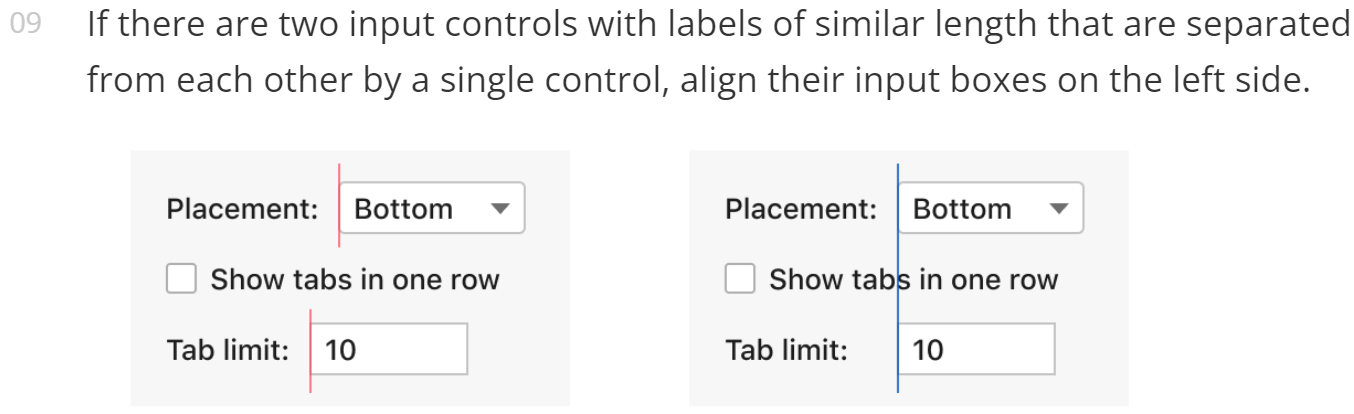
\includegraphics[scale=0.28]{../eng/jbg-09.png}
	}

	\caption{������ ����������������� ����������: ���������, ������������ � ������� �����������}
	\label{form1-structure-layout}
\end{figure}



\begin{figure*}[t]
\begin{verbnobox}[\fontsize{10pt}{10pt}\selectfont]
ordered main_group (
  Label "Type" describes TextEdit "Any" {width=200}
  Label "Owner" describes TextEdit "Anyone" {width=200}
  Label "Has the words" describes TextEdit "Enter words found in the file" {
   width = 400
  }
  Label "Item name" describes
    TextEdit "Enter a term that matches part of the file name" {
      width = 400
    }
  (Label "Location" describes
    (TextEdit "Anywhere" { width = 200 }) dominates
    ordered location_checkboxes (
      Label "In trash"  describes CheckBox in_trash_checkbox
      Label "Starred"   describes CheckBox starred_checkbox
      Label "Encrypted" describes CheckBox encrypted
    )
  )
  Label "Date modified" describes  TextEdit "Any time" {width=200}
  Label "Approvals" describes
    ordered approvals_checkboxes (
      Label "Awaiting my approval" describes CheckBox awaiting_checkbox
      Label "Requested by me" describes CheckBox requestred_checkbox
  )
  Label "Shared to" describes
    TextEdit "Enter a name or email address..." {width=400}
  Label "Follow-ups" describes TextEdit "---" {width=200, height=35}
)
Button "Search" approves^ main_group
Button "Reset" cancels^ main_group
\end{verbnobox}
\caption{�������� ��������� ������� ������ �� ������� Google Drive}
\label{gd_structure}
\end{figure*}

\begin{figure*}[t]
    \begin{subfigure}[t]{.45\textwidth}
        \vspace{-18em}
        \centering
        \begin{minipage}{6cm}
        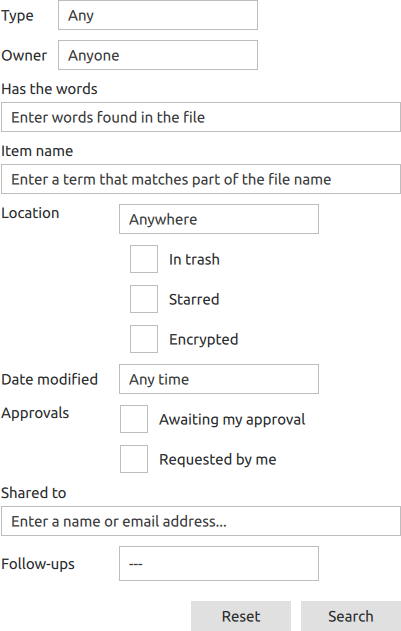
\includegraphics[scale=0.25]{../eng/google-drive-search-setting-output2.png}
        \end{minipage}
        \caption{���� ����� ��������� \enquote{������� �������} ������� ����������, �� ����������� �� �����������}
    \end{subfigure}\hspace{1cm}
    \begin{subfigure}[t]{.45\textwidth}
      \centering
      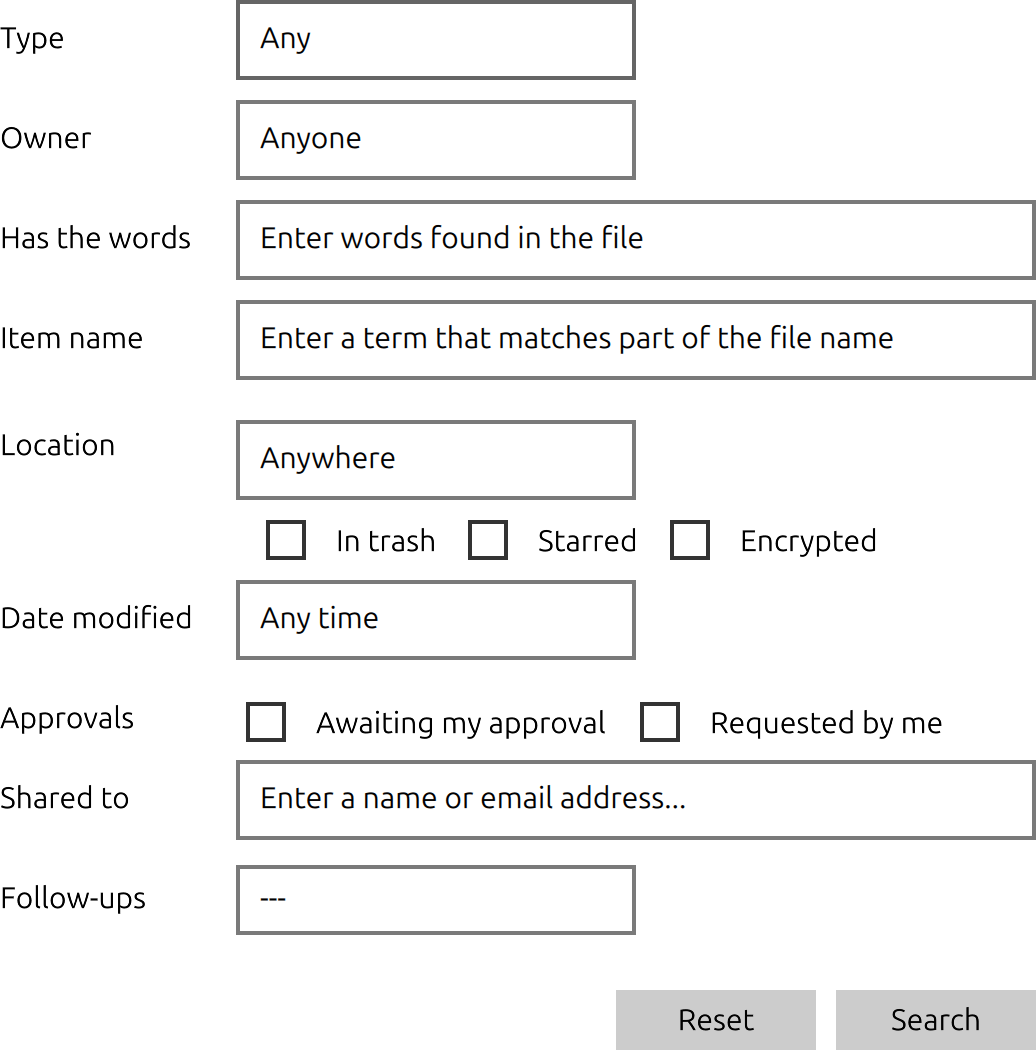
\includegraphics[scale=0.25]{../eng/google-drive-search-setting-output3.png}
      %\vskip17.5mm
      \caption{�� �� �����, �� ��������� ��� ��������  \enquote{������� �������} ���������}
    \end{subfigure}
    \caption{��������������� ������������ ��������� ��� ������� �� Google Drive}
    \label{fig:QMLtwoGuidelines}
\end{figure*}





\begin{figure*}
	\centering
    \begin{tabular}{m{85mm}m{6cm}}
      \begin{lstlisting}[basicstyle=\small]
ordered (
  Label "Short label"
    describes TextEdit "Text 1"
  Label "Loooooong label"
    describes TextEdit "Text 2"
)
      \end{lstlisting} &
      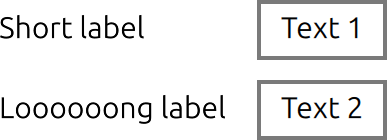
\includegraphics[scale=0.4]{../eng/Example1-Qt-QML.png} \\
      \hline
      \begin{lstlisting}[basicstyle=\small]
ordered (
  Label "Looooong label"
    describes TextEdit "Text 1"
  Label "Medium label"
    describes TextEdit "Text 2"
  Label "Short"
    describes TextEdit "Text 3"
)
      \end{lstlisting} &
      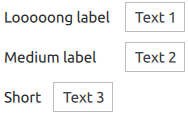
\includegraphics[scale=0.4]{../eng/Example2-Qt-QML.png} \\
      \hline
      \begin{lstlisting}[basicstyle=\small]
ordered (
  Label "Short label"
      describes TextEdit "Text 1"
  Label "Check box label"
      describes CheckBox _
  Label "Looooong label"
      describes TextEdit "Text 2"
)
      \end{lstlisting} &
      \vspace{1em}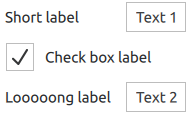
\includegraphics[scale=0.4]{../eng/Example4-Qt-QML.png} \\
      \hline
      \begin{lstlisting}[basicstyle=\small]
ordered (
  Label "L 1"     describes CheckBox _
  Label "Lab 2"   describes CheckBox _
  Label "Label 3" describes CheckBox _
  Label "Label 4" describes CheckBox _
  Label "L 5"     describes CheckBox _
  Label "Lab 6"   describes CheckBox _
)
      \end{lstlisting} &
      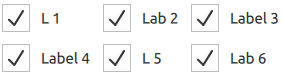
\includegraphics[scale=0.4]{../eng/Example5-Qt-QML.png} \\
    \end{tabular}
    \caption{������� �������� (�����) � ��������������� ������������ (������) � ������ ����������� �� JetBrains}
    \label{fig:evaluation}
  \end{figure*}

\label{lastpage}
\end{document}
